
\chapter{AVALIAÇÃO DA SOLUÇÃO}\label{chap:result}

    Visando validar se o \textit{framework} proposto atende as necessidades dos usurários foi feito uma pesquisa de uso do \textit{framework} com algumas pessoas da área da Programação.
    Através da plataforma \textit{Google Forms} foram aplicados 5 perguntas sobre a experiencia dos usurários com o \textit{framework} em relação ao \textit{Selenium Webdriver}.
    No total, 7 usuários foram selecionados para executar alguns casos de testes e automatização utilizando o \textit{framework}, todos os participantes tinham conhecimentos entre
    básicos e intermediário em \textit{Selenium Webdriver} e os cenários foram executados em computadores com \textit{linux} com o \textit{Python} instalado.
    Com isso foram levantados os seguintes pontos sobre a utilização do mesmo:
    Profissão do Usuário,
    Facilidade de instalação,
    Facilidade de Uso,
    Atende necessidades básicas,
    Atende necessidades avançadas.

    A seguir, serão mostrados e analisado os dados coletados em cada um dos pontos do questionário, este que pode ser encontrado no apêndices deste trabalho.

    \section{Profissão do Usuário}
        Como trata-se de um \textit{framework} de automação de testes foi solicitado um numero maior de profissionais da área de \textit{Testes de Software}.
        Como exemplo, pode ser observado na Figura~\ref{fig:profissao}, mais de 70\% dos usuários são Testadores de Software, enquanto menos de 30\% são
        Desenvolvedores.

        \begin{figure}[H]
            \vspace*{0,2cm}
            \centering
            \caption{Profissões}
            \fbox{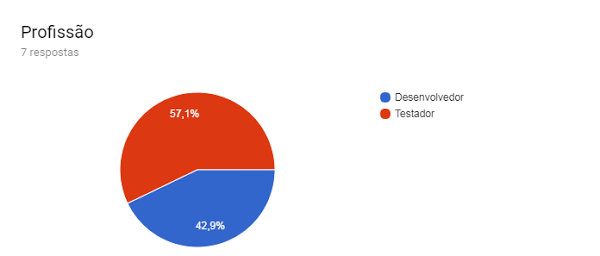
\includegraphics[width=0.8\textwidth]{./04-figuras/profissao}}
            \label{fig:profissao}
        \end{figure}

    \section{Facilidade de instalação}
        Dos usuários na grande maioria consideraram fácil a instalação, como pode ser observado na Figura~\ref{fig:instalacao}. O único ponto a melhorar foi
        que o projeto hoje está disponível apenas pelo repositório do \textit{Github} e não no \textit{PIP}, repositório padrão do \textit{Python}.

        \begin{figure}[H]
            \vspace*{0,2cm}
            \centering
            \caption{Facilidade de instalação}
            \fbox{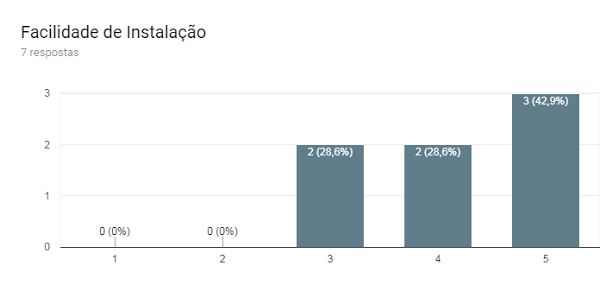
\includegraphics[width=0.8\textwidth]{./04-figuras/instalacao}}
            \label{fig:instalacao}
        \end{figure}

    \section{Facilidade de Usabilidade}

        Em relação a facilidade de uso a grande maioria não teve muitas dificuldades, onde mais de 50\% considerou a usabilidade mediana e o restante de fácil uso,
        como podemos observar na Figura ~\ref{fig:uso}. Onde o maior problema levantado a falta de documentação para verificar todos os comandos de cada classe.

        \begin{figure}[H]
            \vspace*{0,2cm}
            \centering
            \caption{Facilidade de Uso}
            \fbox{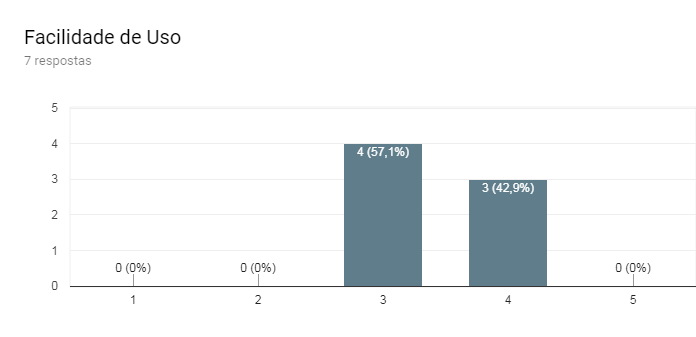
\includegraphics[width=0.8\textwidth]{./04-figuras/uso}}
            \label{fig:uso}
        \end{figure}

    \section{Atende as necessidades básicas}
        As funcionalidades disponíveis do \textit{framework} foram, para a maioria, suficientes para atender as necessidades básicas de criação de um processo de testes.
        Como para a Facilidade de Uso, a documentação também foi um ponto negativo levantado.

          Como pode ser visto na Figura ~\ref{fig:basico}, nenhum usuário classificou com nota 5 que representa representa que o \textit{framework} não atende completamente
          todas as necessidades básicas dos usuários.

        \begin{figure}[H]
            \vspace*{0,2cm}
            \centering
            \caption{Atende necessidades básicas}
            \fbox{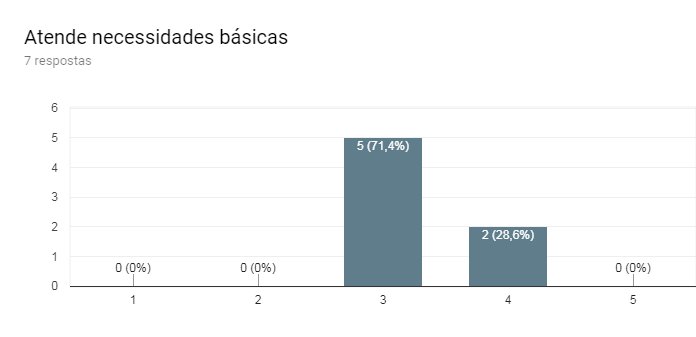
\includegraphics[width=0.8\textwidth]{./04-figuras/basicas}}
            \label{fig:basico}
        \end{figure}

    \section{Atende as necessidades avançadas}
        O \textit{framework} não atingiu as necessidades avançadas. Os usuários tiveram diversos problemas para utilizar múltiplas janelas e elementos renderizados em
        processos assíncronos do \textit{Javascripts}, sendo necessário fazer uso do \textit{Selenium} padrão contido no \textit{framework} para realizar tais tarefas.

          Como pode ser visto na Figura~\ref{fig:avancado}, todos os usuários consideraram que o \textit{Pybot} não atendeu necessidades avançadas.

        \begin{figure}[H]
            \vspace*{0,2cm}
            \centering
            \caption{Atende necessidades avançadas}
            \fbox{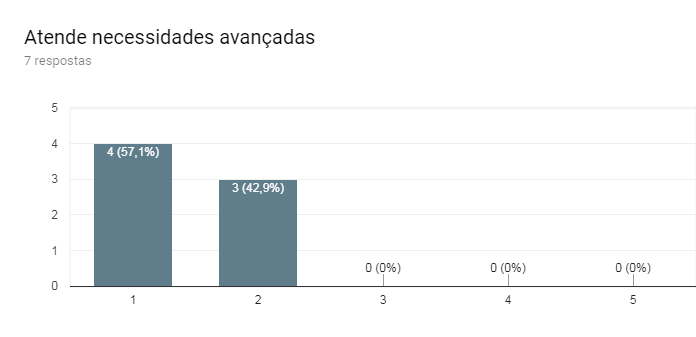
\includegraphics[width=0.8\textwidth]{./04-figuras/avancadas}}
            \label{fig:avancado}
        \end{figure}
